\section{Aufbau und Durchführung}
\label{sec:Durchführung}
In diesem Abschnitt wird zunächst der Aufbau und die Einstellung der verwendeten Messapparatur beschrieben und anschließend die Durchführung des Experimentes dokumentiert.
\subsection{Aufbau der Messapparatur}
In Abbildung \ref{fig:aufbauop} ist der Versuchsaufbau zu sehen:
\begin{figure}[h!]
  \centering
  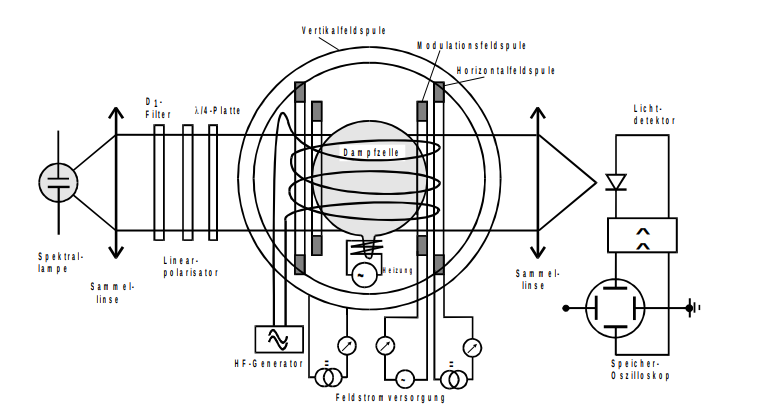
\includegraphics[scale=0.55]{fig/aufbauop.png}
  \caption{Schematische Darstellung der Messapparatur \cite{Anleitung1}}
  \label{fig:aufbauop}
\end{figure}
Der Versuchsaufbau besteht wie oben gezeigt aus einer Rubidium-Spektrallampe, einem D1-Filter, der nur die Wellenlänge $\lambda=\SI{794.9}{\nano\meter}$ durchlässt. Daraufhin wird das Licht mithilfe eines Linearpolarisators und einer $\dfrac{\lambda}{4}$ Platte polarisiert.
Das polarisierte Licht trifft auf eine Dampfzelle, welche sich innerhalb von drei Helmholtzspulen befindet. Zwei davon erzeugen horizontale Magnetfelder. Am Ende fällt das Licht auf einen Detektor.
Zwischen der Spektrallampe und dem Detektor stehen zwei Sammellinsen.
\subsection{Durchführung}
Am Anfang werden die optischen Elemente eingesetzt. Dafür werden diese so justiert, dass der Ausschlag auf dem Galvanometer maximal wird.
Danach wird der Tisch in Nord-Süd Richtung ausgerichtet, um eine Komponente des Erdmagnetfeldes zu kompensieren. Der Versuch wird mit einer schwarzen Decke abgedeckt, da dieser sehr lichtempfindlich ist.
Das Oszilloskop wird auf den X-Y-Modus gestellt. Die Vertikale Helmholtzspule wird so lange variiert, bis der Peak so schmal wie möglich wird, um eine weitere Komponente des Erdmagnetfeldes zu kompensieren.
 Ein Sinusgenerator wird anschließend an das Kontrollgerät angeschlossen und die Frequenz wird von $\SI{100}{\kilo\hertz}$ bis $\SI{1}{\mega\hertz}$ in $\SI{100}{\kilo\hertz}$ Schritten erhöht. Die Resonanzen beider Isotope werden dabei für jede Frequenz gemessen. Die Horizontale Spule wird dann eingestellt, wenn die Peaks der Isotope nicht im angezeigten Bereich liegen.
